\documentclass[conference]{IEEEtran}
% Relatorio incremental do mestrado (formato IEEE conference) - versao enxuta.
% A versao detalhada esta em relatorio-completo.tex.
% Compilar com pdfLaTeX (Overleaf: Menu > Compiler > pdfLaTeX).

\usepackage[utf8]{inputenc}
\usepackage[T1]{fontenc}
\usepackage[brazil]{babel}
\usepackage{cite}
\usepackage{amsmath,amssymb,amsfonts}
\usepackage{graphicx}
\usepackage{booktabs}
\usepackage{multirow}
\usepackage{textcomp}
\usepackage{xcolor}
\usepackage{url}

% Marcador para valores ainda nao obtidos (treinos em execucao)
\newcommand{\pend}{\textcolor{gray}{--}}

\begin{document}

\title{Replicação do \textit{Reflective Gaussian Splatting} para Objetos Reflexivos: Primeiros Resultados e Propostas}

\author{\IEEEauthorblockN{João Pedro Maciel Pimenta}
\IEEEauthorblockA{\textit{Centro de Informática} \\
\textit{Universidade Federal de Pernambuco}\\
Recife, Brasil \\
jpmp3@cin.ufpe.br}
\and
\IEEEauthorblockN{Francisco Paulo Magalhães Simões}
\IEEEauthorblockA{\textit{Centro de Informática} \\
\textit{Universidade Federal de Pernambuco}\\
Recife, Brasil \\
fpms@cin.ufpe.br}
}

\maketitle

\begin{abstract}
Métodos de Gaussian Splatting reconstroem cenas 3D a partir de fotos e as renderizam em tempo real, mas têm dificuldade com objetos espelhados, como metais polidos. O Reflective Gaussian Splatting (Ref-Gaussian) trata esse problema modelando explicitamente o material e a luz refletida. Este relatório descreve o método, aponta uma limitação na forma como ele decide se um reflexo está bloqueado por outra parte do objeto e propõe duas formas de melhorá-la. Como primeiro passo, o código oficial foi executado em um notebook comum e os resultados do artigo foram replicados em duas cenas do conjunto Shiny Blender, com valores próximos aos publicados.
\end{abstract}

\begin{IEEEkeywords}
Gaussian Splatting, superfícies reflexivas, reconstrução 3D, renderização.
\end{IEEEkeywords}

% =====================================================================
\section{Introdução}

O 3D Gaussian Splatting (3DGS)~\cite{kerbl2023} representa uma cena como um grande conjunto de ``manchas'' 3D em formato de elipsoide, chamadas Gaussianas, cada uma com posição, tamanho, cor e transparência. A partir de várias fotos de um objeto, o método ajusta essas Gaussianas até que, projetadas na tela, reproduzam as fotos. O resultado pode ser visto de novos ângulos em tempo real.

O 3DGS funciona mal com objetos espelhados. A cor de cada Gaussiana muda com o ângulo de visão de forma simplificada, o que não é suficiente para representar reflexos nítidos. O método acaba ``pintando'' o reflexo como se fosse geometria atrás da superfície.

O Ref-Gaussian~\cite{yao2025refgaussian} resolve boa parte desse problema e é hoje um dos melhores métodos para objetos reflexivos. Por isso ele foi escolhido como \textit{baseline}, isto é, o método de referência que a dissertação pretende melhorar. Este relatório tem dois objetivos: explicar o método e as propostas de melhoria (Seção~\ref{sec:metodo}) e reproduzir os resultados do artigo antes de qualquer modificação (Seções~\ref{sec:exp} e~\ref{sec:resultados}).

% =====================================================================
\section{Solução Proposta}\label{sec:metodo}

\subsection{Como o Ref-Gaussian funciona}

A Fig.~\ref{fig:pipeline} resume o método. Ele tem quatro ideias principais.

\begin{figure*}[t]
\centering
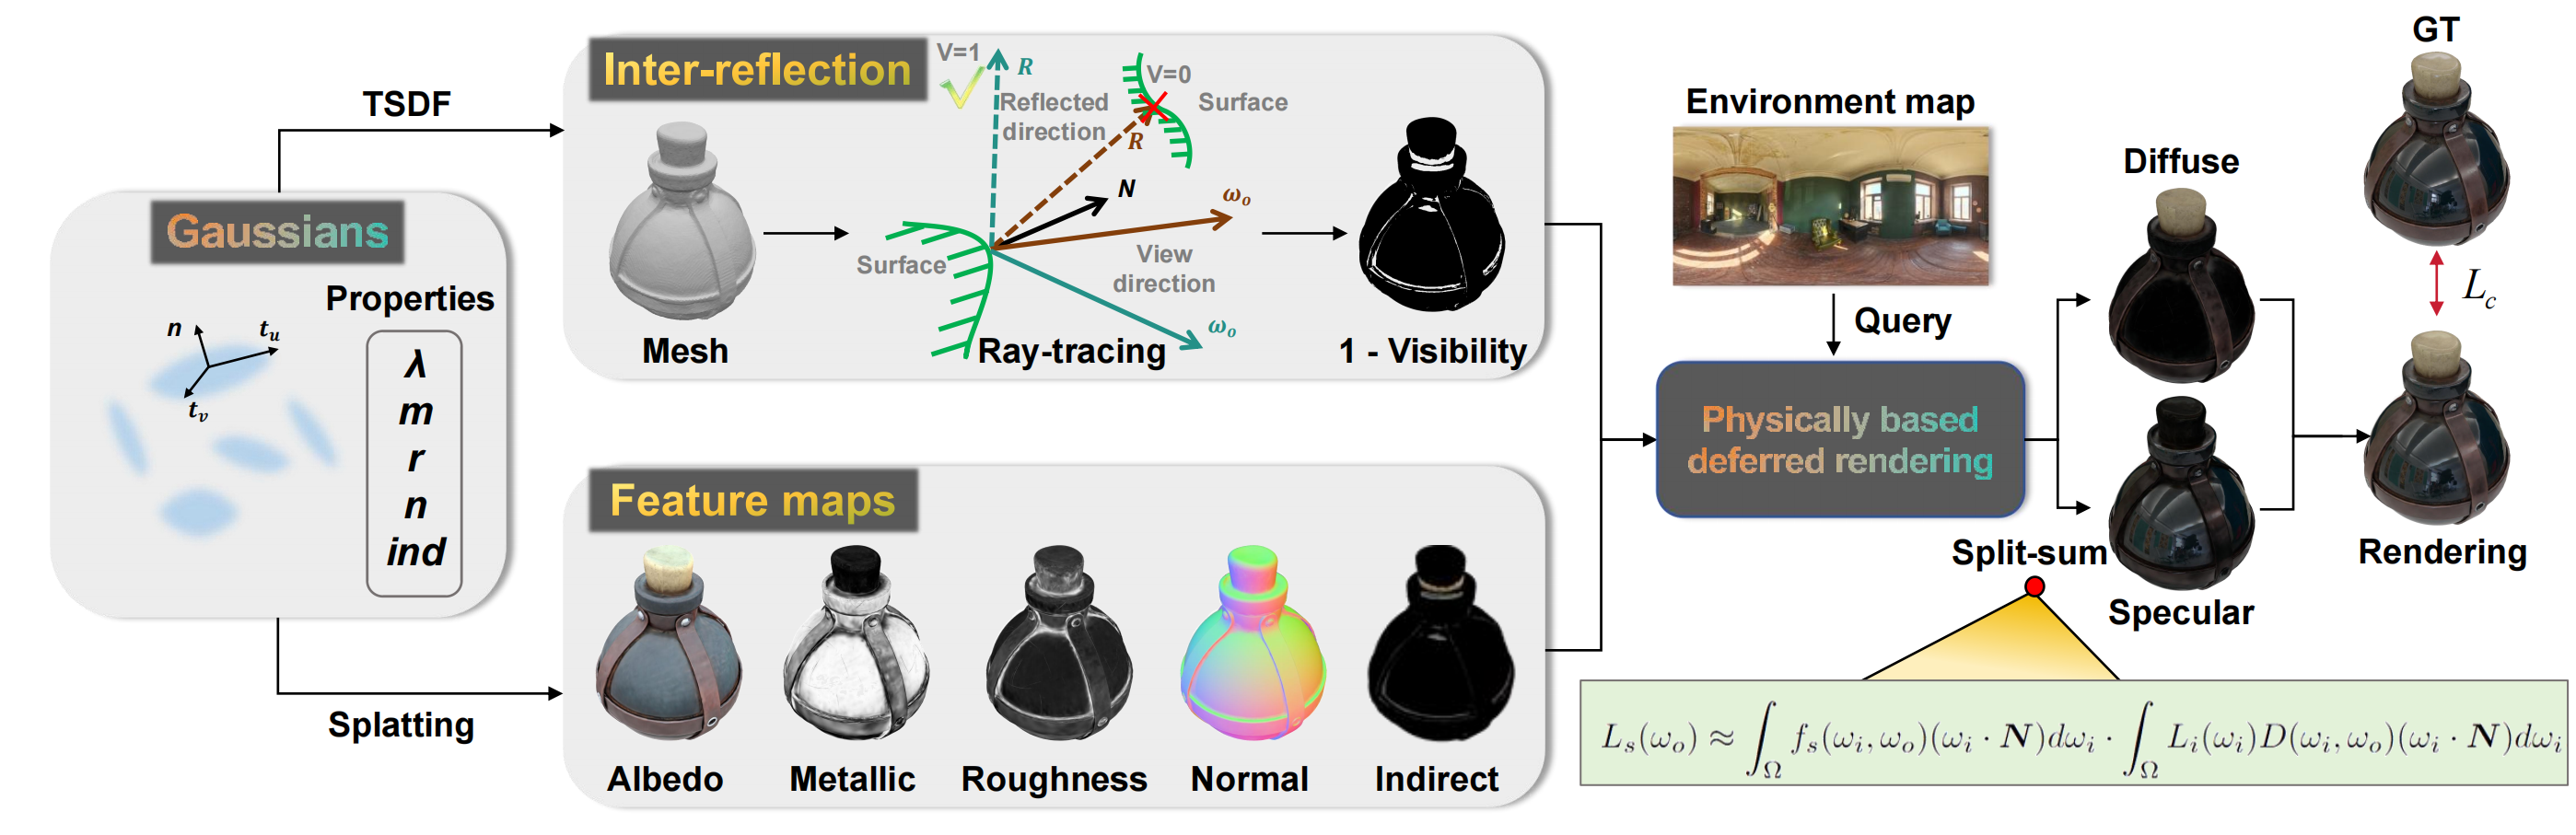
\includegraphics[width=0.92\textwidth]{figs/pipeline_refgaussian.png}
\caption{Visão geral do Ref-Gaussian. As Gaussianas guardam propriedades de material, que são projetadas em mapas por pixel; a cor final é calculada a partir desses mapas, da luz do ambiente e dos reflexos entre partes do objeto. Fonte: Yao et al.~\cite{yao2025refgaussian}.}
\label{fig:pipeline}
\end{figure*}

\textbf{1) Gaussianas achatadas.} Em vez de elipsoides, o método usa discos planos (Gaussianas 2D~\cite{huang2024_2dgs}). Um disco tem uma direção perpendicular bem definida, a \emph{normal}, que diz para onde a superfície ``aponta''. Saber a normal é indispensável para calcular reflexos.

\textbf{2) Material em vez de cor.} Cada disco guarda propriedades físicas de material: a cor base (\emph{albedo}), o quanto o material é metálico (\emph{metalicidade}) e o quanto ele é áspero (\emph{rugosidade}). Um metal polido tem metalicidade alta e rugosidade baixa e reflete como um espelho; um metal escovado tem rugosidade maior e reflete de forma borrada.

\textbf{3) Cálculo da luz por pixel.} Primeiro, as propriedades de todos os discos são projetadas na tela, formando um mapa de material por pixel. Só depois a cor é calculada, uma vez por pixel, usando um modelo físico de reflexão e um mapa da luz que vem do ambiente ao redor do objeto. Isso produz reflexos mais nítidos do que calcular a cor disco a disco.

\textbf{4) Reflexos entre partes do objeto.} Um ponto da superfície pode refletir o ambiente distante ou outra parte do próprio objeto, como a lateral de uma torradeira refletindo a fatia de pão. Para decidir qual dos dois casos acontece, o método lança \emph{um} raio na direção do reflexo e verifica se ele bate no objeto. O resultado é a \emph{visibilidade} $V$, que vale 1 se o raio escapa para o ambiente e 0 se é bloqueado:
\begin{equation}
L_{\text{reflexo}} = V \cdot L_{\text{ambiente}} + (1-V) \cdot L_{\text{objeto}} .
\label{eq:vis}
\end{equation}
Para lançar esse raio, o método precisa de uma malha de triângulos da superfície, que é recalculada a partir das Gaussianas a cada 2 mil iterações de treino.

\subsection{Limitação e propostas}

O próprio artigo aponta uma limitação na Eq.~\eqref{eq:vis}. Um reflexo real não vem de uma única direção, mas de um pequeno ``cone'' de direções, que é mais largo quanto mais áspero é o material. Testar só o raio central é uma aproximação, e os autores observam que ela introduz ruído nas propriedades de material estimadas. Além disso, recalcular a malha periodicamente tem custo e cria uma segunda representação da geometria, separada das Gaussianas.

A partir disso, a dissertação propõe investigar:

\textbf{P1 -- Visibilidade em todo o cone de reflexão.} Lançar alguns raios distribuídos dentro do cone, em vez de um só, e usar a média, $\bar{V} = \frac{1}{K}\sum_{k=1}^{K} V_k$. O número de raios $K$ cresceria com a rugosidade; para um espelho perfeito, $K=1$ recupera o método original.

\textbf{P2 -- Visibilidade sem malha.} Calcular se o raio é bloqueado diretamente a partir das Gaussianas, sem gerar a malha, aproveitando trabalhos recentes de traçado de raios sobre Gaussianas~\cite{moenne2024_3dgrt}.

Uma terceira direção, a extensão para objetos reflexivos em movimento, fica como trabalho futuro.

% =====================================================================
\section{Experimentos}\label{sec:exp}

O objetivo desta etapa é \emph{replicar} o baseline, ou seja, verificar se os resultados do artigo se repetem quando o código é executado por outra pessoa, em outro computador.

\textbf{Ambiente.} Foi usado o código oficial do Ref-Gaussian, sem modificações no método, em um notebook com GPU NVIDIA RTX 4050 (6~GB), Windows~11 e CUDA~11.8. O código foi feito para Linux, e foi necessário ajustar opções de compilação das suas partes em CUDA para que funcionassem no Windows. Esses ajustes estão registrados em scripts no repositório do projeto.

\textbf{Dados.} Usou-se o conjunto Shiny Blender~\cite{verbin2022refnerf}, com seis objetos sintéticos muito reflexivos. Cada objeto tem 100 imagens para treino e 200 para teste, todas com $800\times800$ pixels. Até aqui foram concluídas duas cenas, \textit{toaster} (uma torradeira) e \textit{ball} (uma esfera); as outras quatro estão em andamento.

\textbf{Treino.} Cada cena foi treinada por 50 mil iterações, com as configurações padrão do código oficial. As primeiras 18 mil iterações usam um modo mais simples, que serve para estabilizar a forma do objeto; os reflexos entre partes do objeto são ativados a partir da iteração 20 mil.

\textbf{Métricas.} Cada imagem de teste gerada pelo modelo é comparada com a imagem real usando três métricas comuns na área: PSNR, que mede o erro pixel a pixel (maior é melhor); SSIM, que mede a semelhança de estrutura (maior é melhor); e LPIPS, que mede a diferença percebida por uma rede neural treinada para imitar a percepção humana (menor é melhor).

% =====================================================================
\section{Resultados e Discussão}\label{sec:resultados}

\begin{table*}[t]
\centering
\caption{Replicação do Ref-Gaussian no Shiny Blender: valores do artigo~\cite{yao2025refgaussian} e obtidos neste trabalho. $\Delta$ é a diferença de PSNR em relação ao artigo. ``--'' indica cena ainda em treino.}
\label{tab:replicacao}
\begin{tabular}{llccccccc}
\toprule
Métrica & Origem & Ball & Car & Coffee & Helmet & Teapot & Toaster & Média \\
\midrule
% Linhas geradas por atualizar_resultados.py a partir de ref-gaussian/output/<cena>/metric.txt
\csname @@input\endcsname tab_replicacao.tex
\bottomrule
\end{tabular}
\end{table*}

\begin{figure*}[t]
\centering
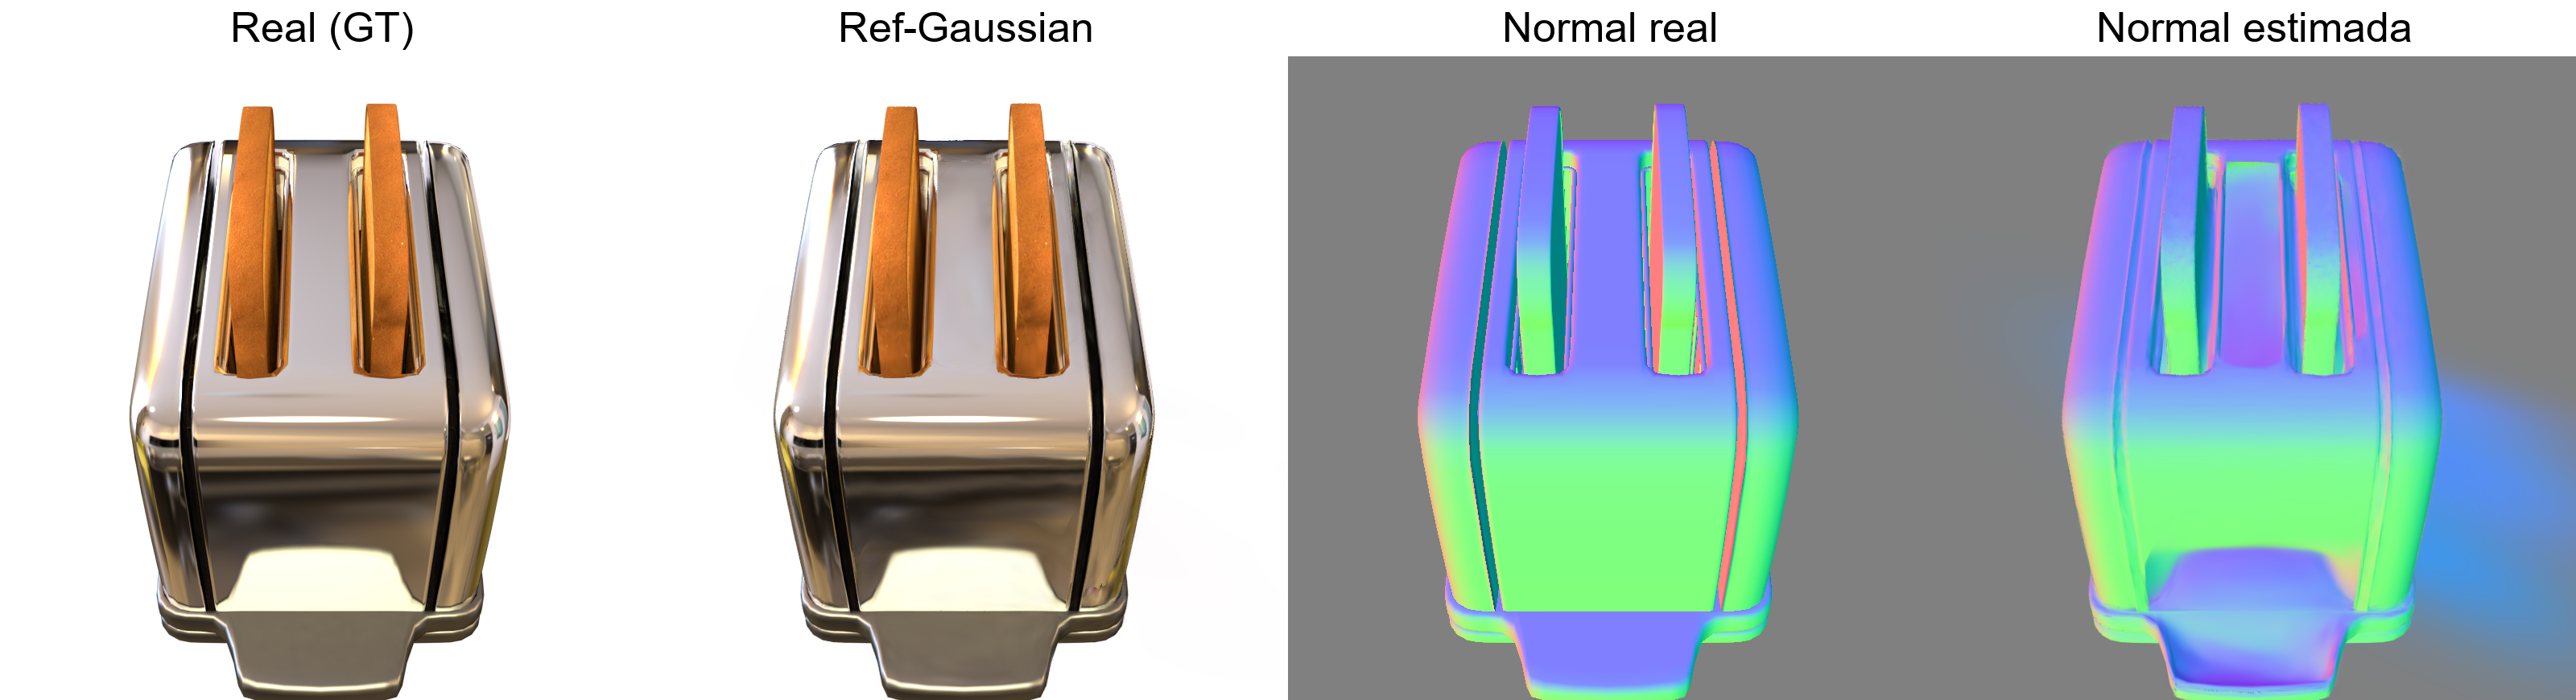
\includegraphics[width=\textwidth]{figs/toaster_qualitativo.png}\\[2pt]
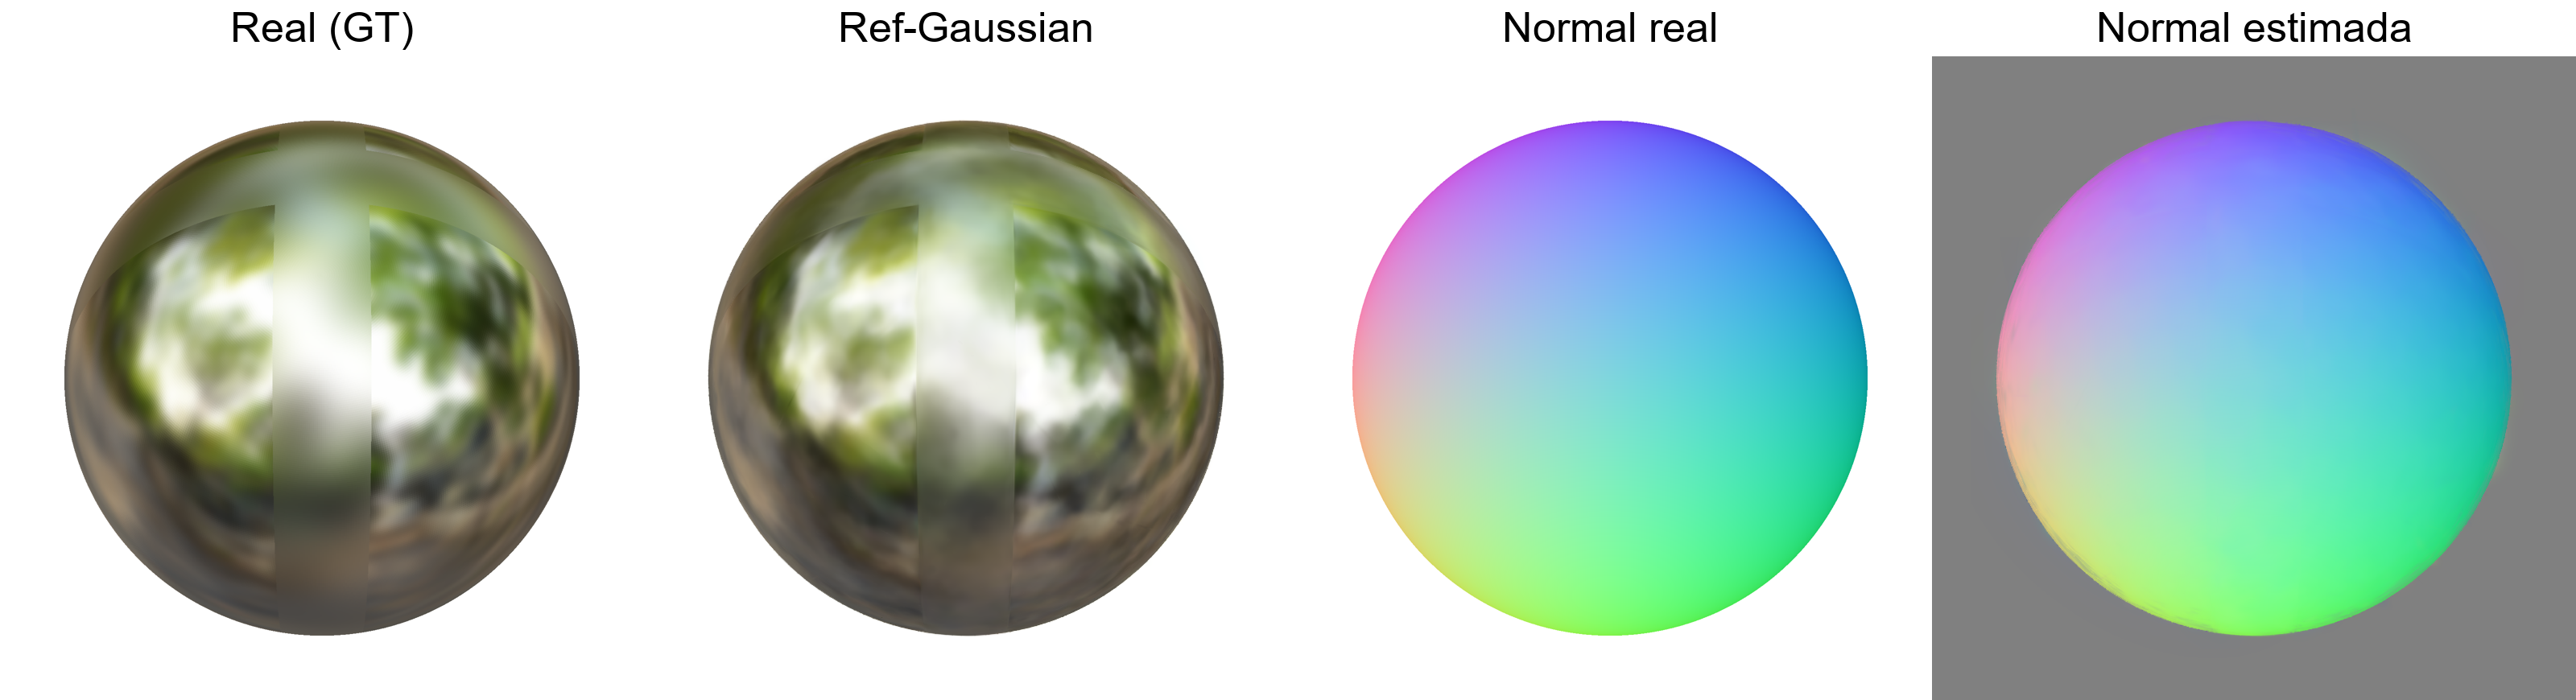
\includegraphics[width=0.8\textwidth]{figs/ball_qualitativo.png}
\caption{Resultados nas cenas \textit{toaster} (acima) e \textit{ball} (abaixo), na primeira imagem de teste. Da esquerda para a direita: imagem real, imagem gerada pelo Ref-Gaussian, normal real e normal estimada (as cores codificam a direção da superfície).}
\label{fig:qualitativo}
\end{figure*}

\begin{figure}[t]
\centering
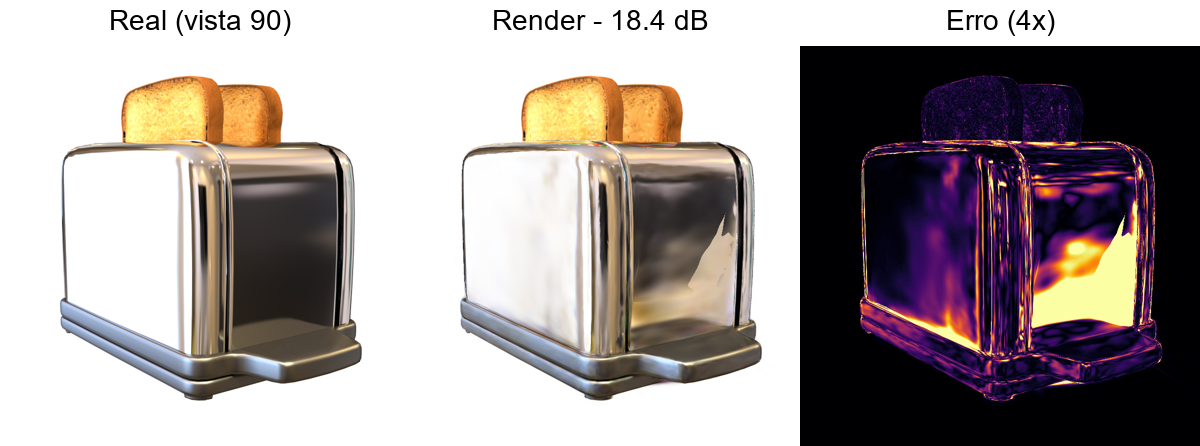
\includegraphics[width=\columnwidth]{figs/toaster_pior.png}
\caption{Pior imagem de teste da \textit{toaster} (18,4~dB): real, gerada e mapa de erro (amarelo indica erro maior). A lateral espelhada, que na foto real reflete uma região escura, aparece clara.}
\label{fig:extremos}
\end{figure}

\textbf{Os resultados do artigo se repetem.} A Tabela~\ref{tab:replicacao} compara os valores obtidos com os publicados. Na \textit{toaster}, o SSIM e o LPIPS são iguais aos do artigo e o PSNR fica 0,54~dB abaixo. Na \textit{ball}, o PSNR fica 0,94~dB abaixo, mas o SSIM e o LPIPS ficam até um pouco melhores. Diferenças dessa ordem são esperadas, porque o treino tem componentes aleatórios e o computador, a GPU e as versões de software são diferentes das usadas pelos autores. Mesmo com essa diferença, os dois resultados continuam acima do melhor método anterior ao Ref-Gaussian segundo o próprio artigo (3DGS-DR~\cite{ye2024dr}).

\textbf{Dá para treinar em um notebook.} O treino levou 1h46min na \textit{toaster} e 1h25min na \textit{ball}. O artigo relata cerca de 35 minutos em uma GPU profissional (NVIDIA A6000). A diferença é esperada, mas mostra que os experimentos da dissertação são viáveis com o equipamento disponível.

\textbf{Os reflexos são bons, a geometria fina nem tanto.} Na Fig.~\ref{fig:qualitativo}, as imagens geradas são muito parecidas com as reais, inclusive nos reflexos. As normais estimadas da torradeira, porém, são mais ``lisas'' que as reais: os frisos finos das laterais quase somem. Na esfera, as normais estimadas coincidem com as reais.

\textbf{A média esconde erros localizados.} Na \textit{toaster}, o PSNR médio é de 27,51~dB, mas varia entre 18,4 e 33,5~dB conforme a imagem de teste, e 32 das 200 imagens ficam abaixo de 25~dB. A Fig.~\ref{fig:extremos} mostra o pior caso. Nessa imagem, a lateral da torradeira deveria refletir algo escuro e próximo, mas aparece clara, como se refletisse o ambiente distante. Isso é exatamente o que aconteceria se o raio de visibilidade da Eq.~\eqref{eq:vis} ``escapasse'' quando deveria ser bloqueado. Ainda é uma hipótese, que será verificada nos próximos passos.

\textbf{Objeto côncavo versus convexo.} A comparação entre as duas cenas reforça essa leitura. A torradeira é \emph{côncava}: tem partes que refletem outras partes dela mesma, e a visibilidade importa. A esfera é \emph{convexa}: nenhum ponto reflete o próprio objeto, então a visibilidade é sempre 1 e a aproximação da Eq.~\eqref{eq:vis} é exata. Na esfera, a qualidade é muito mais uniforme: nenhuma imagem de teste fica abaixo de 31,6~dB. Com só duas cenas, que também diferem em material e iluminação, isso ainda não é uma prova, mas é coerente com a ideia de que a visibilidade é o ponto fraco do método e justifica as propostas P1 e P2.

\textbf{Próximos passos.} (i) Concluir as quatro cenas restantes do Shiny Blender e depois os conjuntos Glossy Synthetic~\cite{liu2023nero} e Shiny Blender Real; (ii) extrair os mapas de visibilidade nas imagens com maior erro, para testar a hipótese acima; e (iii) implementar uma primeira versão de P1 e compará-la com o baseline.

% =====================================================================
\section{Conclusão}

O Ref-Gaussian foi escolhido como ponto de partida da dissertação. O código oficial foi colocado para funcionar em um notebook com Windows, e os resultados do artigo foram reproduzidos nas duas primeiras cenas, com diferenças pequenas. A análise inicial indica que os erros se concentram onde o objeto reflete a si mesmo, o que aponta para a forma como o método calcula a visibilidade dos reflexos. As duas propostas apresentadas, usar mais raios no cone de reflexão e calcular a visibilidade sem malha, atacam exatamente esse ponto.

\begin{thebibliography}{00}
\bibitem{kerbl2023} B. Kerbl, G. Kopanas, T. Leimkühler, and G. Drettakis, ``3D Gaussian splatting for real-time radiance field rendering,'' \textit{ACM Trans. Graph.}, vol. 42, no. 4, 2023.
\bibitem{huang2024_2dgs} B. Huang, Z. Yu, A. Chen, A. Geiger, and S. Gao, ``2D Gaussian splatting for geometrically accurate radiance fields,'' in \textit{Proc. ACM SIGGRAPH}, 2024.
\bibitem{yao2025refgaussian} Y. Yao, Z. Zeng, C. Gu, X. Zhu, and L. Zhang, ``Reflective Gaussian splatting,'' in \textit{Proc. Int. Conf. Learn. Represent. (ICLR)}, 2025.
\bibitem{ye2024dr} K. Ye, Q. Hou, and K. Zhou, ``3D Gaussian splatting with deferred reflection,'' in \textit{Proc. ACM SIGGRAPH}, 2024.
\bibitem{verbin2022refnerf} D. Verbin, P. Hedman, B. Mildenhall, T. Zickler, J. T. Barron, and P. P. Srinivasan, ``Ref-NeRF: Structured view-dependent appearance for neural radiance fields,'' in \textit{Proc. IEEE/CVF Conf. Comput. Vis. Pattern Recognit. (CVPR)}, 2022.
\bibitem{liu2023nero} Y. Liu, P. Wang, C. Lin, X. Long, J. Wang, L. Liu, T. Komura, and W. Wang, ``NeRO: Neural geometry and BRDF reconstruction of reflective objects from multiview images,'' \textit{ACM Trans. Graph.}, vol. 42, no. 4, 2023.
\bibitem{moenne2024_3dgrt} N. Moenne-Loccoz, A. Mirzaei, O. Perel, R. de Lutio, J. M. Esturo, G. State, S. Fidler, N. Sharp, and Z. Gojcic, ``3D Gaussian ray tracing: Fast tracing of particle scenes,'' \textit{ACM Trans. Graph.}, vol. 43, no. 6, 2024.
\end{thebibliography}

\end{document}
